\documentclass[a5paper]{article}
\usepackage[a5paper, top=8mm, bottom=8mm, left=8mm, right=8mm]{geometry}

\usepackage{polyglossia}
\setdefaultlanguage[babelshorthands=true]{russian}

\usepackage{fontspec}
\setmainfont{FreeSerif}
\newfontfamily{\russianfonttt}[Scale=0.7]{DejaVuSansMono}

\usepackage[font=scriptsize]{caption}

\usepackage{amsmath}
\usepackage{amssymb,amsfonts,textcomp}
\usepackage{color}
\usepackage{array}
\usepackage{hhline}
\usepackage{cite}

\usepackage[hang,multiple]{footmisc}
\renewcommand{\footnotelayout}{\raggedright}

\PassOptionsToPackage{hyphens}{url}\usepackage[xetex,linktocpage=true,plainpages=false,pdfpagelabels=false]{hyperref}
\hypersetup{colorlinks=true, linkcolor=blue, citecolor=blue, filecolor=blue, urlcolor=blue, pdftitle=1, pdfauthor=, pdfsubject=, pdfkeywords=}

\usepackage{tabu}

\usepackage{graphicx}
\usepackage{indentfirst}
\usepackage{multirow}
\usepackage{subfig}
\usepackage{footnote}
\usepackage{minted}

\sloppy
\pagestyle{plain}

\title{Диаграммы классов UML}
\author{Юрий Литвинов\\\small{yurii.litvinov@gmail.com}}

\date{25.02.2019г}

\begin{document}

\maketitle
\thispagestyle{empty}

\section{Domain-driven design}

 Domain-Driven Design (или предметно-ориентированное проектирование) --- популярная методология проектирования ПО, которая основана на анализе предметной области и реализации модели предметной области в приложении. Архитектуру в рамках этой методологии предлагается строить не исходя из сиюминутных потребностей реализации, а вокруг ``смыслового ядра'', которое отражает основные сущности реального мира, с которым будет работать программа (или семейство программ).

Модель предметной области выражается прежде всего в коде --- сущности предметной области становятся классами языка программирования, используемого для реализации. Также для обсуждения предметной области с экспертами и для документирования модели часто используются диаграммы.

Немаловажную роль как в создании модели, так и в её ``фиксации'' и улучшении играет ещё и устное общение. Неудачные названия классов или методов, неуклюжие и непонятные описания взаимодействий прекрасно слышны в разговоре и являются поводом для того, чтобы посмотреть на модель ещё раз. Сам естественный язык часто подсказывает правильные архитектурные решения --- что неудивительно, язык сотни лет оттачивался как раз для того, для чего он нужен в DDD --- для передачи сути понятий. Ещё раз напомню, что архитектура --- это больше про понимание программы человеком, а не понимание программы компьютером, так что всякие гуманитарные вещи могут сильно помочь при разработке архитектуры.

Модель определяет \textit{единый язык}, на котором должны общаться все члены команды и эксперты предметной области, которые им помогают. Если какой-то термин зафиксирован как имя класса, использование его синонимов ни в диалогах, ни в документации, ни тем более в коде не допускаются, можно использовать только имя класса. Так же и с методами --- если действию дали название, можно использовать только его, и если это не удобно, название меняют. Это, во-первых, упрощает общение и сопровождение программы, во-вторых, способствует улучшению модели, постоянно её тестируя на предмет неконсистентностей, недопониманий и неоднозначностей.

Модель появляется не только благодаря применению единого языка и последовательного именования всех нужных сущностей, она также ``выкристаллизовывается'' в процессе непрерывного рефакторинга и уточнения. Поскольку программисты редко владеют предметной областью, в которой они решают задачу, построить правильную и хорошую модель предметной области невозможно просто потому, что знаний не хватает. Есть понятие ``переработка знаний'' --- когда программисты строят модель, одновременно активно изучая предметную область. Узнав что-то новое, они включают это в модель, рисуют диаграммы, обсуждают их с экспертами, корректируют модель, и т.д. до тех пор, пока не будет достигнуто достаточное понимание. Цель ``переработки знаний'' --- не получить понимание, достаточное для реализации программы, а понять принципы, по которым работает сама предметная область, а уже потом написать программу. Интересно, что если модель хороша и программисты неплохи в выделении абстракций, то в процессе переработки знаний кое-чему научиться могут и эксперты.

Таким образом можно эффективно работать с незнакомой предметной областью. Если вас попросят разработать архитектуру непонятно чего (а в домашке попросят, и не один раз), начать следует не с рисования диаграмм классов (это не более чем инструмент), а с анализа предметной области и построения её модели, выражаемой в том числе в виде диаграмм классов UML. То есть методология проектирования (в частности, DDD) позволяет понять, откуда брать эти самые диаграммы классов.

Дальнейший рассказ является, по сути, кратким пересказом первой главы книги Эрика Эванса, ``Предметно-ориентированное проектирование. Структуризация сложных программных систем''. М., ``Вильямс'', 2010, 448 стр. Если есть время, лучше её прочитать, если нет, то про неё дальше будет рассказ поподробнее.

\section{Переработка знаний}

Рассмотрим анализ предметной области на примере из книжки. Перед Эриком Эвансом была поставлена задача разработать приложение для проектирования печатных плат. При этом он, естественно, ничего не знал про печатные платы и сроки проекта не позволяли ему глубоко погружаться в эту область. У Эванса был доступ к инженерам, которых он мог использовать в качестве экспертов, но они ничего не понимали в программировании. Попытка получить с них подробное ТЗ привела к тому, что там надо было считать данные из файла, отсортировать их, дополнить какими-то другими данными, вывести и сгенерировать отчёты.

Как известно, качество ПО определяется не его соответствием ТЗ, а удовлетворением пользователей, так что делать по такому ТЗ Эванс, естественно, не стал. Однако в описании функций приложения упоминались отчёты, а в них постоянно встречалось понятие ``цепь'' --- проводник, соединявший произвольное количество компонентов на плате. Так у нас появилось первое приближение модели предметной области:

\begin{center}
	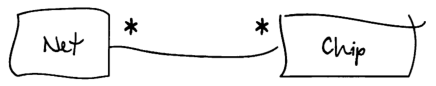
\includegraphics[width=0.6\textwidth]{netClasses.png}
\end{center}

И некоторый набор неформальных диаграмм объектов для перебора разных сценариев, например:

\begin{center}
	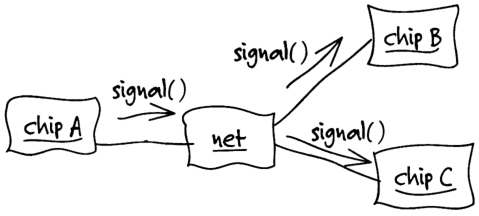
\includegraphics[width=0.6\textwidth]{netObjects.png}
\end{center}

В ходе обсуждения со специалистами выяснилось, что компонент --- это не обязательно chip, а они используют термин component instance. Пришлось объяснить инженерам, почему цепь сама выглядит как компонент. Заодно выяснилось, что у элементов есть выводы (pins), каждый вывод принадлежит только одному элементу и подключается только к одной цепи. При этом у каждой цепи есть топология, то есть правила, по которым цепь соединяет свои элементы. Получилась уточнённая модель:

\begin{center}
	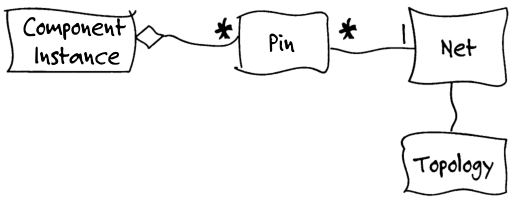
\includegraphics[width=0.7\textwidth]{topology.png}
\end{center}

Тут Эванс решил выбрать конкретную задачу, с которой можно было бы начать, и, поговорив с инженерами, решил, что будет делать сначала программное прозванивание цепи --- отслеживаине распространения сигнала с целью найти слишком долгие задержки в распространении. В ходе общения выяснилось, что сигнал передаётся по цепи от вывода к выводу и внутри компонента по каким-то своим законам, которые мы не хотим моделировать, но знаем, с какого выхода на какой выход каждый конкретный компонент передаёт сигнал. Добавим в модель понятие ``push'' (проталкивание сигнала внутри компонента) и таблицу пушей, привязанную к компоненту:

\begin{center}
	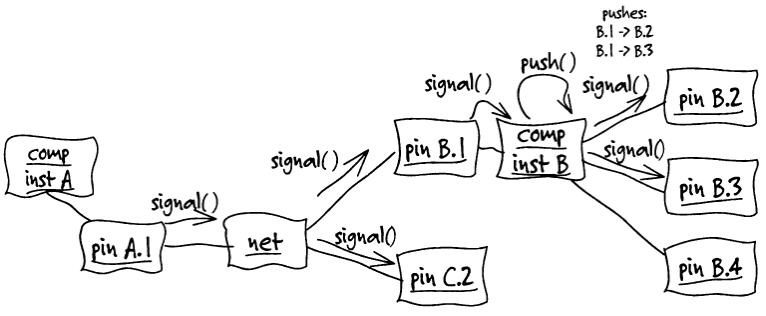
\includegraphics[width=0.9\textwidth]{signals.png}
\end{center}

Теперь можно смоделировать прозванивание, добавив сигналу в качестве параметра количество его перепосылок по цепи:

\begin{center}
	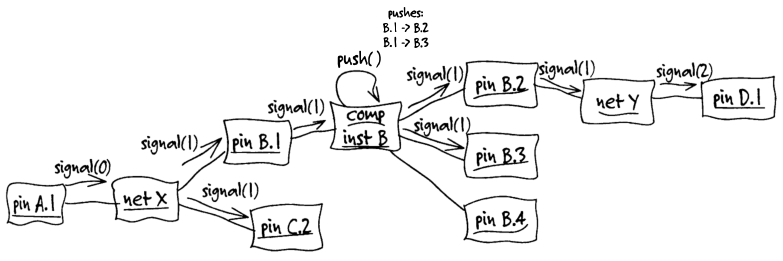
\includegraphics[width=\textwidth]{probeSimulation.png}
\end{center}

Смотря на эту модель, мы понимаем, что что-то тут не то, надо хранить таблицу пушей для каждого компонента. Спросив у инженеров, узнаём, что вовсе нет --- у каждого компонента есть тип, и компоненты одного типа все ведут себя одинаково, хотя их может быть много на плате. Таким образом, таблицу можно хранить только для типа компонента, и каждый компонент должен знать свой тип:

\begin{center}
	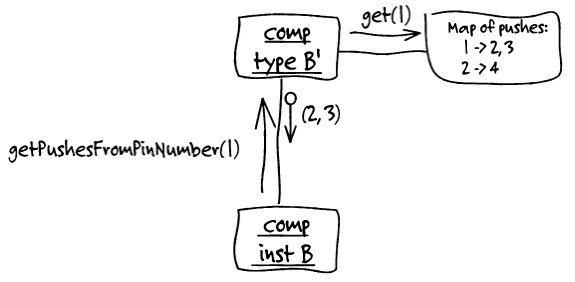
\includegraphics[width=0.7\textwidth]{types.png}
\end{center}

Инженеры из этой диграммы мало что поняли, но согласились, что всё выглядит примерно так. Теперь у нас есть полное представление о том, что происходит, и мы можем нарисовать модель для прозванивания, но внезапно вспоминаем про топологию цепи и узнаём у инженеров, что для прозванивания топология не используется. Выкидываем её из модели, потому что хоть такое понятие в предметной области есть, для создаваемой функциональности оно нерелевантно, мы про него ничего не знаем и всегда можем вернуть это понятие в модель, когда в нём таки возникнет необходимость. Итого, получилась вот такая диаграмма классов:

\begin{center}
	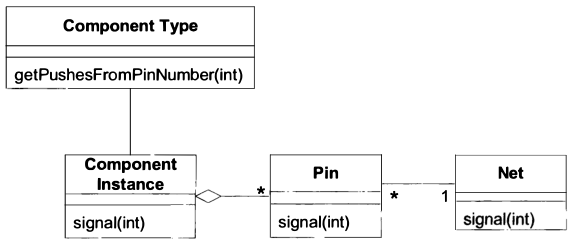
\includegraphics[width=0.8\textwidth]{finalModel.png}
\end{center}

\section{Выводы}

Из рассмотренного примера можно сделать следующие выводы, касающиеся анализа предметной области по канонам Domain-Driven Design-а.

\begin{itemize}
	\item Детали реализации не участвуют в модели. По двум соображениям сразу --- во-первых, они непонятны экспертам (а с экспертами надо согласовывать модель н акаждом этапе), во-вторых, они перегружают модель и заставляют думать о том, о чём можно подумать и на этапе реализации.
	\item Должно быть можно общаться, пользуясь только именами классов и методов. Если использовать имя класса как термин неудобно, это означает либо то, что он называется неудачно и его надо переименовать, либо что это на самом деле два класса и его надо явно разделить.
	\item Не нужные для текущей задачи сущности предметной области не должны быть в модели. В примере на какой-то промежуточной диаграмме появлялось понятие ``топология'', но мы про него ничего не знаем и в решении задачи прозванивания оно никак не участвует, так что его убрали из модели. Зато те сущности, которые для решения задачи нужны, должны быть проработаны подробно.
	\item Могут быть скрытые сущности, которые следует выделить явно и явно сделать частью модели. При этом надо объяснить экспертам их предназначение. Примеры таких сущностей --- это фабрики объектов, репозитории, иногда даже ограниччения на состояние системы --- в предметной области их, как правило, нет, но они важны для реализации и их следует ввести явно в модель и в единый язык.
	\item Диаграммы объектов могут быть очень полезны как средство анализа. В примере мы их рисовали примерно поровну с диаграммами классов.
\end{itemize}

\end{document}